\section{Results}
We can not look into the results of our work and show how we can create our different variations of the game. As we have already discussed, we can give the player three different abilities and likewise we can give the boss two different abilities, but we can also choose not to have a boss. We have succeeded in being able to create these variation, unfortunately as discussed in the '\nameref{Room}' subsection we have been unable to create variations with weather effects. We can thus create \textbf{nine} different variations.

\begin{figure}[H]
	\centering
	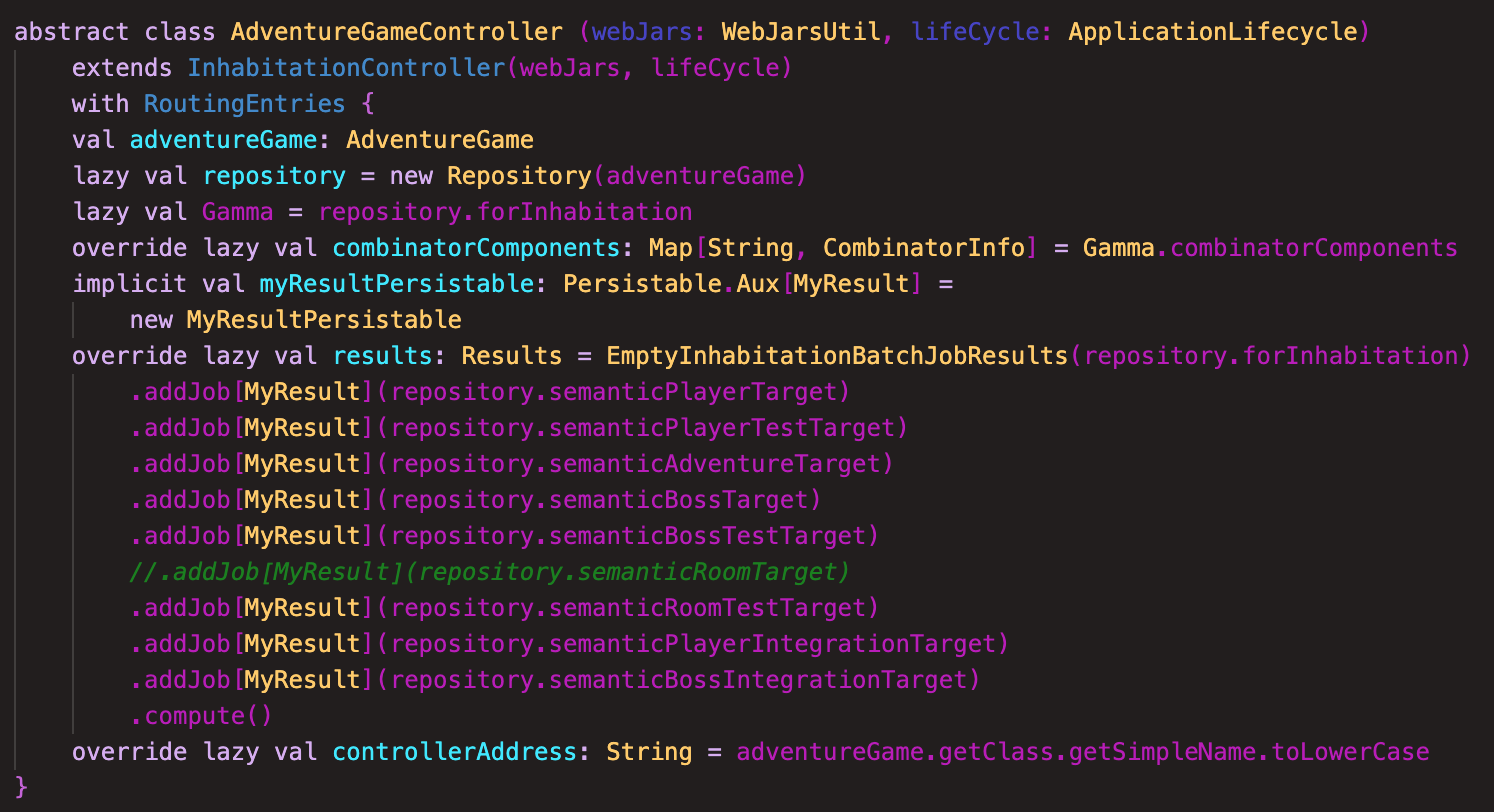
\includegraphics[width=\linewidth]{Materials/Results/AdventureController}
	\caption{In the \textit{AdventureGameController} we can see what jobs we are scheduling and thus what we want synthesized.}
	\label{Controller}
\end{figure}
In \autoref{Controller} we see \textit{AdventureGameController} in which we add the jobs we want done. Each job correspond to a synthesis we want done, and so if we are only interested in creating a player we could remove the other jobs. As seen we have removed \textit{semanticRoomTarget} as it will not finish.\\
To alter the variation we synthesize we need to look at a concrete class which extends our \textit{AdventureGame} class. We can here look at \textit{AdventureGameVersion1} which is seen in \autoref{version1}. We here see the player having the fireball ability, the boss having the damage reduction ability, and the possible weather effects being blizzard.\\

\begin{figure}
	\centering
	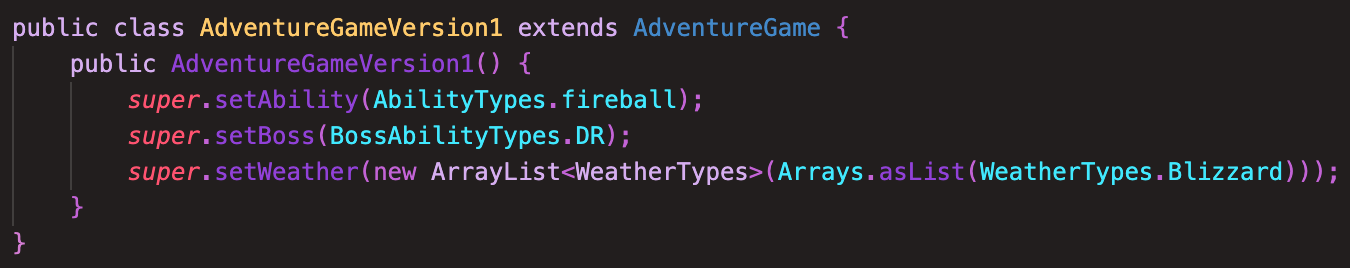
\includegraphics[width=\linewidth]{Materials/Results/AdventureVariation}
	\caption{By setting the \textit{AdventureGame} fields we can create different variation of our game. Here is shown a variation where the player has the fireball, the boss has the damage reduction ability and the possible weather effects would be blizzard.}
	\label{version1}
\end{figure}
As the room can not be synthesized we can unfortunately not showcase a variation with a boss. This is because the room has a combinator adding three methods if we are synthesizing a variation with a boss which the boss rely on. Instead we can check the files which is being synthesized and that way verify the boss is being synthesized correctly. \\
In the following we will showcase that the initial application can be synthesized and played. This however, is because we do not need any changes to the room in the initial application and thus we can use the template file in the project for the room. One could say we have not succeeded in synthesizing the initial application, as the intention was to synthesize the room and we have not.\\
As we start the game we see that we can not hit other players in the room with us. This is because we need the knife to attack with, as we do not have the fireball in the initial application. With the knife we can now begin stabbing both other players, but also the evil customer monster. The concept for hitting the 'Wicked Witch' is the same, but here we need the water. As this is all there is to the game in the initial application our showcase is done.